%TGC: WWg WWZ
%QGC: WWZg WWgg WWWW WWZZ
Processes involving two final state gauge bosons are of particular interest for testing the predictive power of the SM.
Due to the non-Abelian nature of the EWK interaction, the corresponding gauge bosons are allowed to self-interact.
This results in triple and quartic couplings of gauge bosons (TGCs and QGCs, respectively).
The SM allowed TGCs are the $WW\gamma$ and $WWZ$ vertices, and the QGCs predicted by the model include $WWZ\gamma$, $WW\gamma\gamma$, $WWZZ$, and $WWWW$.
These vertices are accessible via a number of production modes at hadron colliders, including vector boson fusion and scattering (VBF and VBS, as in Figure~\ref{fig:theory_vbf_vbs}).
The LHC in particular has provided the first opportunity to observe some of these vertices, such as the $WW\gamma\gamma$ QGC via the $W\gamma\gamma$ final state~\cite{2015.wgg}, or the $WWWW$ QGC via same-sign $W^{\pm}W^{\pm}$ production~\cite{2014.ssww-8tev-atlas}.
Precise measurements of these processes can be compared to the theoretical predictions, and deviations can point to deficiencies in the prediction, such as needing an additional order in $\alpha_s$ in the calculation, or even hints at new physics, like anomalous gauge couplings\footnote{In the SM, the TGCs and QGCs are fixed by the electromagnetic coupling constant $\alpha$ and the electroweak mixing angle $\theta_W$.  In many Beyond the Standard Model scenarios, these couplings are modified by additional contributions.}~\cite{2017.anomalous-tgc-lhc}.

\begin{figure}[htbp]
  \centering
  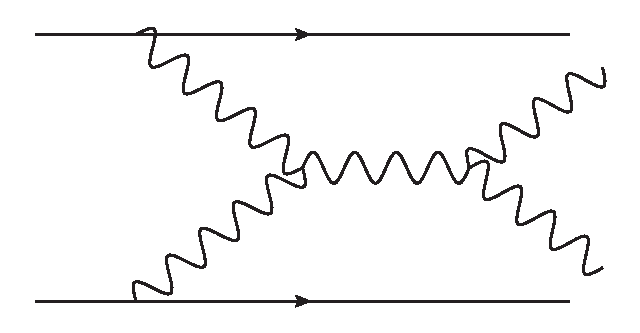
\includegraphics[height=.13\textheight]{figs/theory/vbf}\hspace{20pt}
  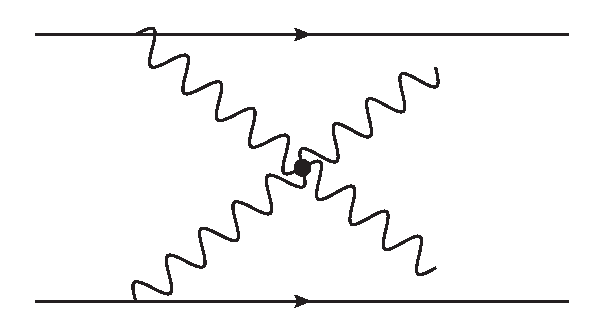
\includegraphics[height=.13\textheight]{figs/theory/vbs}
  \caption{Vector boson fusion involving triple gauge couplings (left) and vector boson scattering involving a quartic gauge coupling (right).}
  \label{fig:theory_vbf_vbs}
\end{figure}

Diboson interactions also make up one of the most sensitive tests of EWSB.
Aside from the top quark, the EWK bosons have the strongest coupling to the Higgs mechanism, as there are several production diagrams involving the exchange of a Higgs boson, including those in Figure~\ref{fig:theory_higgs}.
In this instance, VBS processes are particularly important as the Higgs unitarizes the scattering amplitude~\cite{1977.ben-lee-weak-interactions-physrevd} (this particular aspect will be explored in more detail in the context of same-sign $W^{\pm}W^{\pm}$ scattering in Section~\ref{ssww13tev:vbs_theory}).
Since the Higgs boson has only recently been discovered, it has not yet been extensively tested, and there could still be deviations in the EWSB mechanism that may manifest in the VBF and VBS measurements~\cite{2017.multiboson-at-lhc}.

\begin{figure}[htbp]
  \centering
  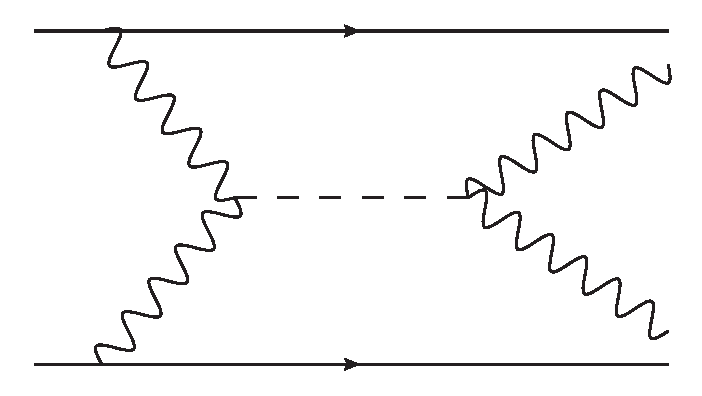
\includegraphics[width=.3\textwidth]{figs/theory/higgs_s}\hspace{20pt}
  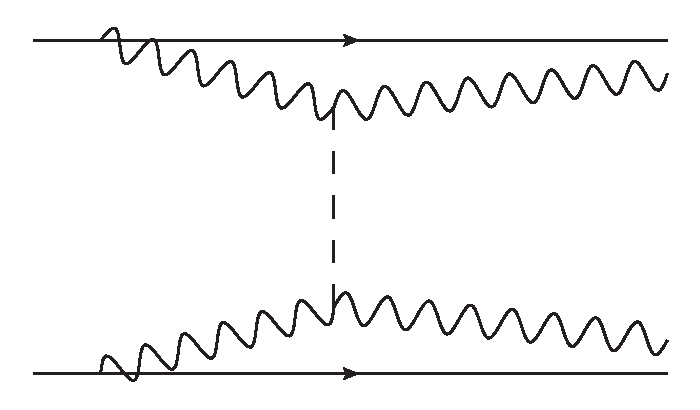
\includegraphics[width=.3\textwidth]{figs/theory/higgs_t}
  \caption{Diboson diagrams involving the $s$-channel (left) and $t$-channel (right) exchanges of a Higgs boson.}
  \label{fig:theory_higgs}
\end{figure}

%An alternative scenario involves anomalous couplings~\cite{2017.anomalous-tgc-lhc}.
%In the SM, the TGCs and QGCs are fixed by the electromagnetic coupling constant $\alpha$ and the electroweak mixing angle $\theta_W$.
%However, in many Beyond the Standard Model (BSM) scenarios, these couplings are modified by additional BSM contributions.
%In this case, the SM Lagrangian is considered to be one component of an overall effective Lagrangian
